%\documentclass{sigplanconf}

\documentclass[12pt]{article}
%\documentclass{llncs}
\usepackage{amsmath, amssymb, fancyvrb, multirow, color, relsize}

%%%%%%%%%%%%%%%%%%%%%%%%%%%%%%%%%%%%%
%%%%%%%%%%%% TECH REPORT %%%%%%%%%%%%
%%%%%%%%%%%%%%%%%%%%%%%%%%%%%%%%%%%%%
%Check if we are compiling under latex or pdflatex
\ifx\pdftexversion\undefined
  \usepackage[dvips]{graphics}
\else
  \usepackage[pdftex]{graphics}
\fi

\usepackage{fullpage,cmu-titlepage2}
\usepackage{times}
\usepackage{rotating}
\usepackage{tabularx}
\usepackage[
%backref controls whether the bibliography has a list of backreferences
%to where the citaiton is used
%backref,
pageanchor=true,
plainpages=false,
pdfpagelabels, % makes the status line page labels the same as latex ones
bookmarks,
bookmarksnumbered,
pdfborder=0 0 0,
pdfpagemode=UseOutlines]{hyperref}
\usepackage{draftstamp}
\usepackage{subfigure}

%\usepackage{multirow}
\usepackage{amsmath,hyperref}
\hypersetup{
    colorlinks,%
    citecolor=blue,%
    filecolor=blue,%
    linkcolor=blue,%
    urlcolor=blue
}
\usepackage{amssymb,verbatim}
\usepackage{fix2col,listings,fancyvrb}
\usepackage{multicol}
\usepackage{graphicx,epsfig}
\usepackage{caption}
\usepackage{stmaryrd}
\usepackage{setspace}
\usepackage{ulem}
\usepackage{newlfont}
\usepackage{epsfig,graphics}
\usepackage{fancybox}
\usepackage{listings}
\usepackage{caption}
\usepackage{graphicx,epsfig}
\usepackage{caption}
\usepackage{makeidx}
\usepackage{listings}
\lstset{
  basicstyle=\ttfamily,
  breaklines=true,
  columns=fullflexible,
  escapeinside = ||,
  breakindent=0pt}
\makeindex

\usepackage{algorithm}
\usepackage{algpseudocode}
\usepackage{hyperref}
\hypersetup{
    colorlinks,%
    citecolor=blue,%
    filecolor=blue,%
    linkcolor=blue,%
    urlcolor=blue
}


%\usepackage[ruled,lined,boxed,commentsnumbered,linesnumbered]{algorithm2e}

\setcounter{secnumdepth}{3}
\setcounter{tocdepth}{2}

\newcommand\bookepigraph[4]{
\vspace{1em}\hfill{}\begin{minipage}{#1}{\begin{spacing}{0.9}
\small\noindent\textit{#2}\end{spacing}
\vspace{1em}
\hfill{}{#3}\\

\vspace{-1em}\begin{flushright}{#4}\end{flushright}}\vspace{2em}
\end{minipage}}

\newcommand{\dom}{\mbox{dom}}

\newcommand\epigraph[3]{
\vspace{1em}\hfill{}\begin{minipage}{#1}{\begin{spacing}{0.9}
\small\noindent\textit{#2}\end{spacing}
\vspace{1em}
\hfill{}{#3}}\vspace{2em}
\end{minipage}}

\newcommand\anonymousepigraph[2]{
\vspace{1em}\hfill{}\begin{minipage}{#1}{\begin{spacing}{0.9}
\small\noindent\textit{#2}\end{spacing}}
\vspace{1em}
\end{minipage}}

\newcommand{\len}{\mathit{len}}
\newcommand{\poly}{\mathsf{poly}}
\newcommand{\N}{\mathbb{N}}
\newcommand{\R}{\mathbb{R}}
\newcommand{\D}{\mathbb{D}}
\newcommand{\cf}{\mathsf{CF}}
\newcommand{\be}{\mathsf{BE}}
\newcommand{\fe}{\mathbb{F}^{[\underline{e}, \overline{e}]}_{\beta,p}}
\newcommand{\rad}{\mathrm{rad}}


\newcommand{\flow}{\mathsf{flow}}
\newcommand{\jump}{\mathsf{jump}}
\newcommand{\inv}{\mathsf{inv}}
\newcommand{\init}{\mathsf{init}}
\newcommand{\guard}{\mathsf{guard}}
\newcommand{\reset}{\mathsf{reset}}
\newcommand{\reach}{\mathsf{Reach}}
\newcommand{\unsafe}{\mathsf{unsafe}}

\newcommand{\safe}{\mathsf{safe}}
\newcommand{\p}{\mathsf{P}}
\newcommand{\np}{\mathsf{NP}}
%\newcommand{\dom}{\mathrm{dom}}


\newcommand\tupleof[1]{\left\langle #1 \right\rangle}
\newcommand\vI{\vec{I}}
\newcommand\va{\vec{a}}
\newcommand\vb{\vec{b}}
\newcommand\vc{\vec{c}}
\newcommand\vd{\vec{d}}
\newcommand\ve{\vec{e}}
\newcommand\vl{\vec{l}}
\newcommand\vu{\vec{u}}
\newcommand\vx{\vec{x}}
\newcommand\vy{\vec{y}}
\newcommand\trp[1]{#1^{{}^{\mbox{\sc{t}}}}}
\newcommand{\lrf}{\mathcal{L}_{\mathbb{R}_{\mathcal{F}}}}
%\usepackage{wrapfigure}

%\doublespacing


\title{Delta-Complete Reachability Analysis (Part I)}
\author{Sicun Gao \and Soonho Kong \and Edmund M. Clarke}

\abstract{
We give a new framework for safety verification of nonlinear hybrid systems, based on delta-decidability of first-order logic formulas over the real numbers. We use expressive logic formulas (which can contain nonlinear ODEs with no analytic solutions) to encode bounded model checking and invariant-based reasoning. Based on the encoding, we solve bounded reachability and invariant validation problems using delta-complete decision procedures. Such techniques allow us to take into account of robustness properties of a system under delta-bounded numerical perturbations. This report describes Part I of the work, focusing on basic definitions and bounded reachability problems. 
}
\keywords{Hybrid Systems, Reachability, Bounded Model Checking}

\trnumber{CMU-CS-13-131}
%\arpasupport{fox}
\support{This research was sponsored by the National Science Foundation grants
no. CNS1330014, no. CNS0926181 and no. CNS0931985, the GSRC under
contract no. 1041377, the Semiconductor Research Corporation under
contract no. 2005TJ1366, and the Office of Naval Research under award
no. N000141010188.}

\begin{document}
\renewcommand*{\thepage}{title-\arabic{page}}
\maketitle
\renewcommand*{\thepage}{\arabic{page}}


\section{Introduction}
%We will show that our recent work on $\delta$-decisions of logic formulas over the real numbers~\cite{} leads to a new verification framework for general hybrid systems. The new framework bypasses much of the well-known theoretical difficulty without weakening verification results, and shows promising experimental results on complex nonlinear benchmarks. 

Formal verification is difficult for hybrid systems with nonlinear dynamics and complex discrete control~\cite{DBLP:conf/emsoft/Alur11,DBLP:conf/lics/Henzinger96}. Few modern techniques from hardware and software verification have seen much success on hybrid systems, because these techniques are all highly dependent on scalable logic solvers. To apply them on hybrid systems, we have to solve logic formulas over the real numbers with (often a large number of) nonlinear functions, which is highly challenging both theoretically and practically. 

In recent work~\cite{DBLP:conf/lics/GaoAC12,DBLP:conf/cade/GaoAC12}, we have shown that logic formulas over the real numbers become much easier to solve when we shift our focus from the standard decision problem to the {\em $\delta$-decision problem}: Given an arbitrary positive rational number $\delta$, we ask if a logic formula is false or {\em $\delta$-true}. The latter answer can be given if the formula {\em would become true} under $\delta$-bounded numerical perturbations on its constant terms. The $\delta$-decision problem is decidable, with reasonable complexity, for bounded first-order sentences over the reals with arbitrary Type 2 computable functions, such as polynomials, trigonometric functions, and Lipschitz-continuous ODEs~\cite{CAbook}. 

This series of reports describes how we use $\delta$-decidability over the reals to develop a new framework for hybrid system verification.

First, $\delta$-decidability results enable the use of an expressive first-order logic signature, which we denote as $\lrf$, to represent general nonlinear hybrid systems. Here, $\lrf$ allows the use of arbitrary Type 2 computable real functions, which, for instance, include nonlinear ODEs that only need to be numerically solvable. Almost all existing classes of hybrid systems that have been studied in the literature can be defined through restrictions on $\lrf$. 

Next, bounded model checking and invariant-based reasoning techniques for $\lrf$-representable hybrid systems are naturally expressed as decision problems for $\lrf$-formulas. The key observation is that, when we shift to solving the $\delta$-decision problem for these formulas, the verification results are not weakened. This motivates the definition of {\em $\delta$-strengthened} versions of the verification techniques. For instance, with $\delta$-strengthened bounded model checking, we always obtain one of the following answers:
\begin{itemize}
\item {Safe} (bounded): The system does not violate the safety property within a bounded time, and a bounded unrolling depth (for discrete mode changes). 
\item {$\delta$-Unsafe}: Under some $\delta$-perturbation on its $\lrf$-representation, the system would violate the safety property. 
\end{itemize}
Thus, when the procedure returns ``safe", it is a precise answer and no error is involved. On the other hand, when we choose a small enough $\delta$, a system that is ``$\delta$-unsafe" exhibits robustness problems. Realistic hybrid systems interact with the physical world and it is impossible to avoid slight perturbations. Thus, under $\delta$-perturbations and should indeed be regarded as unsafe. Note that such robustness problems can not be discovered by solving the precise decision problem. In short, the framework turns numerical errors into stronger verification results. 

It follows from $\delta$-decidability that $\delta$-strengthened bounded reachability and invariant validation are computable for general nonlinear hybrid systems, which stands in sharp contrast to the standard undecidability of reachability of simple systems. Moreover, after bypassing the difficulties with exact real computations, we gain a better understanding of intrinsic properties of hybrid systems. For instance:
\begin{itemize}
\item There exists a three-layer complexity hierarchy for bounded reachability, which depends on the use of mode invariants and nondeterministic flows. 
\item The search for sound and complete rules for exact checking of invariants is a major challenge, while switching to the $\delta$-strengthened version allows a direct logical encoding. 
\end{itemize} 
This report focuses on basic definitions and theoretical results regarding bounded reachability.

%The paper is organized as follows. In Section~\ref{review} we review the first-order language $\lrf$ and $\delta$-decidability results, and define $\lrf$-representations of hybrid systems in Section~\ref{language}. We then define and study the bounded $\delta$-reachability problem in Section~\ref{main}, and show experimental results in Section~\ref{experiments}.



%\paragraph{Related Work} Franzle's work.

\section{$\lrf$-Representations of Hybrid Automata}\label{review}


\subsection{$\lrf$-Formulas}
We will use a logical language over the real numbers, written as $\lrf$, that allows arbitrary {\em computable real functions}. Computability of real functions is a notion well-developed in Computable Analysis~\cite{CAbook}. Intuitively, a real function is computable if it can be numerically simulated up to an arbitrary precision. For the purpose of this paper, it suffices to know that almost all the functions that are needed in describing hybrid systems are computable: polynomials, exponentiation, logarithm, trigonometric functions, and also the solution functions of Lipschitz-continuous ordinary differential equations. Compositions of computable functions are computable. This, as we will show, makes $\lrf$ very powerful and can express almost any realistic hybrid system.

Formally, $\lrf = \langle \mathcal{F}, > \rangle$ represents the first-order signature over the reals with the set $\mathcal{F}$ of computable real functions, which contains all the functions mentioned above. Note that constants are included as 0-ary functions. $\lrf$-formulas are evaluated in the standard way over the corresponding structure $\mathbb{R}_{\mathcal{F}}= \langle \mathbb{R}, \mathcal{F}^{\mathbb{R}}, >^{\mathbb{R}}\rangle$. It is not hard to see that we can put any $\lrf$-formula in a normal form, such that its atomic formulas are of the form $t(x_1,...,x_n)>0$ or $t(x_1,...,x_n)\geq 0$, with $t(x_1,...,x_n)$ composed of functions in $\mathcal{F}$. This follows from the fact that $t(\vec x)=0$ can be written as $-|t(\vec x)|\geq 0$, $t(\vec x)<0$ as $-t(\vec x)>0$, and $t(\vec x)\leq 0$ as $-t(\vec x)\geq 0$. Also, negations in front of atomic formulas can be eliminated by replacing $\neg t(\vec x) > 0$ with $-t(\vec x)\geq 0$, and $\neg t(\vec x)\geq 0$ with $-t(\vec x)>0$. To avoid extra preprocessing of formulas, we can explicitly define $\mathcal{L}_{\mathcal{F}}$-formulas as follows.
\begin{definition}[$\lrf$-Formulas]
Let $\mathcal{F}$ be a collection of computable real functions. We define:
\begin{align*}
t& := x \; | \; f(t(\vec x)), \mbox{ where }f\in \mathcal{F} \mbox{ (constants are 0-ary functions)};\\
\varphi& := t(\vec x)> 0 \; | \; t(\vec x)\geq 0 \; | \; \varphi\wedge\varphi
\; | \; \varphi\vee\varphi \; | \; \exists x_i\varphi \; |\; \forall x_i\varphi.
\end{align*}
In this setting $\neg\varphi$ is regarded as an inductively defined operation
which replaces atomic formulas $t>0$ with $-t\geq 0$, atomic formulas $t\geq 0$
with $-t>0$, switches $\wedge$ and $\vee$, and switches $\forall$ and $\exists$.
Implication $\varphi_1\rightarrow\varphi_2$ is defined as $\neg\varphi_1\vee\varphi_2$.
\end{definition}
For any $\lrf$-formula $\varphi$ with $n$ free variables, we write $\llbracket \varphi\rrbracket = \{\vec a\in \mathbb{R}^n: \varphi(\vec a)\mbox{ is true over }\langle\mathbb{R},\mathcal{F}^{\mathbb{R}}, >^{\mathbb{R}}\rangle\}.$ If $\varphi$ is a sentence (no free variables), we use the standard notation $\mathbb{R}\models\varphi$ to denote that $\varphi$ is true over $\mathbb{R}$.
\begin{definition}[Bounded Quantifiers]
The bounded quantifiers $\exists^{[u,v]}$ and $\forall^{[u,v]}$ are defined as
\begin{align*}
\exists^{[u,v]}x.\varphi &=_{df}\exists x. ( u \leq x \land x \leq v \wedge
\varphi),\\
\forall^{[u,v]}x.\varphi &=_{df} \forall x. ( (u \leq x \land x \leq v)
\rightarrow \varphi),
\end{align*}
where $u$ and $v$ denote $\lrf$ terms, whose variables only
contain free variables in $\varphi$ excluding $x$. 
\end{definition}
%We say a sentence is {\em bounded} if it only contains bounded quantifiers.
\begin{definition}[Bounded $\lrf$-Sentences]
A {\em bounded $\lrf$-sentence} is
$$Q_1^{[u_1,v_1]}x_1\cdots Q_n^{[u_n,v_n]}x_n\;\psi(x_1,...,x_n),$$
where $Q_i^{[u_i,v_i]}$ are bounded quantifiers, and $\psi(x_1,...,x_n)$ is a
quantifier-free $\lrf$-formula.
\end{definition}


\subsection{$\delta$-Perturbations and $\delta$-Decidability}
\begin{definition}[$\delta$-Variants]\label{variants}
Let $\delta\in \mathbb{Q}^+\cup\{0\}$, and $\varphi$ an
$\lrf$-formula of the form
$$\varphi: \ Q_1^{I_1}x_1\cdots Q_n^{I_n}x_n\;\psi[t_i(\vec x, \vec y)>0;
t_j(\vec x, \vec
y)\geq 0],$$ where $i\in\{1,...k\}$ and $j\in\{k+1,...,m\}$. The {\em
$\delta$-weakening} $\varphi^{\delta}$ of $\varphi$ is
defined as the result of replacing each atom $t_i > 0$ by $t_i >
-\delta$ and $t_j \geq 0$ by $t_j \geq -\delta$. That is,
$$\varphi^{\delta}:\ Q_1^{I_1}x_1\cdots Q_n^{I_n}x_n\;\psi[t_i(\vec x, \vec
y)>-\delta; t_j(\vec x,
\vec y)\geq -\delta].$$
It is clear that $\varphi\rightarrow\varphi^{\delta}$~(see \cite{DBLP:conf/lics/GaoAC12}).
\end{definition}
In~\cite{DBLP:conf/lics/GaoAC12,DBLP:conf/cade/GaoAC12}, we have proved that the following $\delta$-decision problem is decidable. This result serves as the basis of our framework.
\begin{theorem}[$\delta$-Decidability]\label{delta-decide} Let $\delta\in\mathbb{Q}^+$ be
arbitrary. There is an algorithm which, given any bounded $\varphi$,
correctly returns one of the following two answers:
\begin{itemize}
\item ``$\delta$-$\mathsf{True}$'': $\varphi^{\delta}$ is true.
\item ``$\mathsf{False}$'': $\varphi$ is false.
\end{itemize}
Note when the two cases overlap, either answer is correct.
\end{theorem}
We now turn to the complexity issues. Informally, a real function is (uniformly) $\mathsf{P}$-computable ($\mathsf{PSPACE}$-computable) over a compact domain, simply if it can be numerically computed within polynomial-time (polynomial-space). Details can be found in~\cite{kobook,DBLP:conf/lics/GaoAC12}. It suffices to know that many common real functions are $\mathsf{P}$-computable, which includes the polynomials, $\exp$, $\log$, $\sin$, etc. The intuition is that they can be effectively approximated, for instance with Taylor expansions. It is also shown that the solution functions of $\mathsf{P}$-computable Lipschitz-continuous differential equations are $\mathsf{PSPACE}$-computable~\cite{kobook} (in fact, $\mathsf{PSPACE}$-complete~\cite{Kawamura09}).

To state the complexity of the $\delta$-decision problems, we recall the definition of the relativized complexity classes and polynomial hierarchy. The polynomial hierarchy, relativized to a set $A$, is defined as $\mathsf{(\Sigma_0^P)^A= (\Pi_0^P)^A=P^A}$, $\mathsf{(\Sigma_{k+1}^P)^A= NP^{(\Sigma_k^P)^A}}$, and $\mathsf{(\Pi_{k+1}^P)^A=coNP^{(\Sigma_{k}^P)^A}}$.
\begin{theorem}[Complexity~\cite{DBLP:conf/lics/GaoAC12}]\label{compmain}
Let $S$ be a class of $\lrf$-sentences, such that for any $\varphi$ in $S$, the functions in $\varphi$ are in complexity class $\mathsf{C}$. Then, for any $\delta\in \mathbb{Q}^+$, the $\delta$-decision problem for bounded $\Sigma_n$-sentences in $S$ is in $\mathsf{(\Sigma_n^P)^C}$.
\end{theorem}







\subsection{Hybrid Automata with {\large$\lrf$}-Representations}\label{language}

Hybrid automata extend finite automata with continuous dynamics. We first show that $\lrf$-formulas can be used as a concise and natural representation of general hybrid systems.

\begin{definition}[$\lrf$-Representation]\label{lrf-definition}
A hybrid automaton in $\lrf$-representation is a tuple
\begin{multline*}
H = \langle X, Q, \{{\flow}_q(\vec x, \vec x_0, t): q\in Q\},\{\inv_q(\vec x): q\in Q\},\\ \{\jump_{q\rightarrow q'}(\vec x, \vec x'): q,q'\in Q\}, \{\init_q(\vec x): q\in Q\}\rangle,
\end{multline*}
where $X\subseteq \mathbb{R}^n$ for some $n\in \mathbb{N}$, and $Q=\{q_1,...,q_m\}$ is a finite set of modes, and the other components are sets of quantifier-free $\lrf$-formulas.
\end{definition}

Almost all hybrid systems studied in the existing literature can be defined by restricting the signature $\mathcal{F}$. For instance,

\begin{example}[Linear and Polynomial Hybrid Automata] Let $\mathcal{F}^{\mathrm{lin}} = \{+\}\cup \mathbb{Q}$ and $\mathcal{F}^{\mathrm{poly}}=\{\times\}\cup\mathcal{F}^{\mathrm{lin}}$ (Rational numbers are considered as 0-ary functions.) In existing literature, we say $H$ is a {\em linear hybrid automaton} if it has an $\mathcal{L}_{\mathbb{R}_{\mathcal{F}^{\mathrm{lin}}}}$-representation, and a {\em polynomial hybrid automaton} if it has an $\mathcal{L}_{\mathbb{R}_{\mathcal{F}^{\mathrm{poly}}}}$-representation.
\end{example}

\begin{example}[Nonlinear Bouncing Ball]
The bouncing ball is a standard hybrid system model. The point of the example is to emphasize that nonlinear components can be written directly in the $\lrf$-representation.
$$H_{BB}= \langle X, Q, \flow, \jump, \inv, \init\rangle$$
where
\begin{itemize}
\item $X = \mathbb{R}^2$ and $Q = \{q_u, q_d\}$.
\item $\flow_{q_u}(x_0, v_0, x_t, v_t, t)$:
$$(x_t = x_0 + \int_0^{t} v(s) ds) \wedge (v_t = v_0 + \int_0^t g(1-\beta v(s)^2) ds)$$
$\flow_{q_d}(x_0, v_0, x_t, v_t, t)$:
$$(x_t = x_0 + \int_0^{t} v(s) ds) \wedge (v_t = v_0 + \int_0^t g(1+\beta v(s)^2) ds)$$
where
$\beta$ is a constant. Note that the integration terms define Type 2 computable functions, and can be directly used in $\lrf$-formulas.
\item $\jump_{q_d \rightarrow q_u} (x, v, x', v')$:
$$x= 0 \wedge v' = v\cdot\exp(-\frac{c\pi}{2m\omega_d}) \wedge x'=x$$
$\jump_{q_u \rightarrow q_d} (x, v, x', v')$:
$$v= 0 \wedge x' = x \wedge v' = v$$
\item $\init_{q_d}: x=10 \wedge v=0$.
\item $\inv_{q_d}: x>=0 \wedge v>=0$ and $\inv_{q_u}: x>=0 \wedge v<=0$.  
\end{itemize}
\end{example}

\subsection{Hybrid Trajectories}

Trajectories of hybrid systems combine continuous flows and discrete jumps. This motivates the use of a hybrid time domain, with which we can keep track of both the discrete changes and the duration of each continuous flow.

\begin{definition}[Hybrid time domain]
A {\em hybrid time domain} is a subset of
 $\mathbb{N}\times \mathbb{R}$ of the form
$$T_m=\{(i, t): i<m \mbox{ and } t\in [t_i, t_i']\mbox{ or }[t_i, +\infty)\},$$
where $m\in \mathbb{N}\cup\{+\infty\}$, $\{t_i\}_{i=0}^m$ is an
increasing sequence in $\mathbb{R}^+$, $t_0= 0$, and $t_i'=t_{i+1}$.
\end{definition}
%\begin{figure}[h!]
%\begin{center}
%\includegraphics[width= 7cm]{hybrid_time.pdf}
%\end{center}
%\caption{Hybrid time domain}
%\end{figure}
\begin{definition}[Hybrid Trajectories]
Let $X\subseteq\mathbb{R}^n$ be an Euclidean space and $T_m$ a hybrid
time domain. A {\em hybrid trajectory} is any continuous function $\xi: T_m
\rightarrow X.$
 \end{definition}
To define trajectories of hybrid systems, we use a labeling function $\sigma_{\xi,H}(i)$ to map a step $i$ to the corresponding discrete mode in $H$. In each mode, the system flows continuously following the dynamics defined by $\flow(q, \vec x_0, t)$. Note that $(t-t_k)$ is the actual duration in the $k$-th mode. When a switch between two modes is performed, it is required that $\xi(k+1, t_{k+1})$ is updated from the exit value $\xi(k, t_k')$ in the previous mode, following the jump conditions.

\begin{definition}[Trajectories of a Hybrid Automaton]\label{trajec}
Let $H$ be a hybrid automaton, $T_m$ a hybrid domain, and $\xi: T_m\rightarrow X$ a hybrid trajectory.
We say that $\xi$ is {\em a trajectory of $H$ of discrete depth $m$}, written as $\xi\in \llbracket H \rrbracket$, if there
exists a {\em labeling function} $\sigma_{\xi,H}: \mathbb{N}\rightarrow Q$ such
that:
\begin{itemize}
\item For some $q\in Q$, $\sigma_{\xi,H}(0) = q$ and $\mathbb{R}_{\mathcal{F}}\models \init_{q}(\xi(0,0))$.
\item For any $(i, t)\in T_m$, $\mathbb{R}_{\mathcal{F}}\models \inv_{\sigma_{\xi,H}(i)} (\xi(i,t))$.
\item For any $(i,t)\in T_m$, 
\begin{itemize}
\item When $i=0$, $\mathbb{R}_{\mathcal{F}}\models\flow_{q_0}(\xi(0,0), \xi(0,t), t).$
\item When $i = k+1$, where $0<k+1<m$, we have
\begin{eqnarray*}
& &\mathbb{R}_{\mathcal{F}}\models\flow_{\sigma^H_{\xi}(k+1)}(\xi(k+1, t_{k+1}), \xi(k+1, t), (t - t_{k+1})),\\
& &\mathbb{R}_{\mathcal{F}}\models \jump_{\sigma_{\xi,H}(k)\rightarrow\sigma_{\xi,H}(k+1)}(\xi(k, t_k'), \xi(k+1,t_{k+1})).
\end{eqnarray*}
\end{itemize}
\end{itemize}
We can write the time domain $T_m$ of $\xi$ as $T(\xi)$.
\end{definition}
%We write $\llbracket H\rrbracket$ to denote the set of all the trajectories of $H$.
\begin{remark}[$\jump$ vs $\inv$] The jump conditions specify when $H$ {\em may}  switch to another mode. The invariants (when violated) specify when $H$ {\em must} switch to another mode. They will lead to different logical encodings in reachability analysis. 
\end{remark}


\subsection{$\delta$-Perturbations}

The key benefit of using $\lrf$-representations for describing hybrid automata is that operations on the logic formulas can be directly transferred.
\begin{definition}[$\delta$-Perturbations] Let $\delta\in\mathbb{Q}^+\cup\{0\}$. Suppose $H = \langle X, Q, \flow, \jump, \inv, \init\rangle$ is an $\lrf$-representation of hybrid system $H$. We define the {\em $\delta$-weakening} of $H$ as
$$H^{\delta} = \langle X, Q, \flow^{\delta}, \jump^{\delta}, \inv^{\delta},
\init^{\delta}\rangle.$$
\end{definition}

\begin{example}
The $\delta$-weakening of the bouncing ball automaton has its component formulas by their $\delta$-weakening. For instance, $\flow_{q_u}^{\delta}(x_0, v_0, x_t, v_t, t)$ is
$$|x_t - (x_0 + \int_0^{t} v(s) ds)|\leq \delta \wedge |v_t - (v_0 + \int_0^t g(1-\beta v(s)^2) ds))|\leq \delta,$$
and $\jump_{q_d \rightarrow q_u}^{\delta} (x, v, x', v')$ is 
$$|x|\leq \delta \wedge |v' - v\cdot\exp(-\frac{c\pi}{2m\omega_d})|\leq \delta \wedge |x'-x|\leq \delta.$$
\end{example}

It is important to note that the notion of $\delta$-perturbations is a purely syntactic one (defined on the description of hybrid systems), instead of a semantic one (defined on the trajectories). Note that the syntactic perturbations naturally lead to a semantic over-approximation of $H$ in the trajectory space:
\begin{proposition} For any $H$ and $\delta\in\mathbb{Q}^+\cup\{0\}$, $\llbracket H\rrbracket\subseteq \llbracket H^{\delta}\rrbracket.$
\end{proposition}
\begin{proof}
Let $\xi\in \llbracket H\rrbracket$ be any trajectory of $H$. Following
Definition~\ref{variants}, for any $\lrf$ sentence $\varphi$, we have
$\varphi\rightarrow\varphi^{\delta}$. Since
$\xi$ satisfies the conditions in Definition~\ref{trajec}, after replacing each
formula by their $\delta$-weakening, we have $\xi\in \llbracket H^{\delta}\rrbracket$.
\end{proof}

\begin{proposition}
The $\delta$-weakening of any hybrid automaton is nondeterministic.
\end{proposition}


\subsection{Reachability}


The safety/reachability problem for hybrid systems can now be formally stated as follows.

\begin{definition}[Reachability]\label{reachability}\index{Reachability}
Let $H$ be an $n$-dimensional hybrid automaton, and $U$ a subset of its state
space $Q\times X$.  We say {\em $U$ is reachable by $H$}, if there exists
$\xi\in\llbracket
H \rrbracket$ with its time domain $T$ and labeling function
$\sigma_{\xi}^H$, such that there exists $(i,t)\in T$ satisfying
$(\sigma^H_{\xi}(i), \xi(i,t))\in U.$
\end{definition}
The bounded reachability problem for hybrid systems is defined by restricting
the continuous components and time duration to a bounded domain, and the number
of discrete transitions to a finite number.


\begin{definition}[Bounded Reachability]
Let $H$ be an $n$-dimensional hybrid automaton, whose continuous state space
$X$ is a bounded subset of $\mathbb{R}^n$. Let $U$ be a subset of its state
space. Let $k\in \mathbb{N}$ and $M \in \mathbb{R}$. The {$(k,M)$-bounded
reachability problem} asks whether there exists
$\xi\in\llbracket H \rrbracket$ with its time domain $T(\xi)$ and labeling function
$\sigma_{\xi}$, such that there exists $(i,t)\in T(\xi)$ with $i\leq k$, $t=
\sum_{i=0}^k t_i$ where $t_i \leq M$, and $(\sigma_{\xi}(i), \xi(i,t))\in U.$
\end{definition}
%\begin{notation}When $M\in\mathbb{R^+}$, we write $T^M$ to denote a time domain whose continuous fragments are bounded by $M$, i.e., for each $(i,t_i)\in T^M$, $t_i\leq M$.\end{notation}
\begin{remark}
By ``step", we mean the number of discrete jumps. We say $H$ can reach $U$ in $k$ steps, if there exists $\xi\in\llbracket H\rrbracket$ that contains $k$ discrete jumps, entering and exiting the continuous flows in $k+1$ modes.
\end{remark}
In the seminal work of \cite{DBLP:conf/rex/AlurD91,DBLP:conf/hybrid/AlurCHH92},
it is shown that the bounded reachability problem for simple classes of hybrid
automata is undecidable. Note that a common restriction in the existing study is that all constants are rational numbers, which does not need to be the case in our definitions. 
\section{Bounded Reachability}\label{main}

In this section we study the bounded $\delta$-reachability problem and how to solve it practice. At the core of our framework is the correspondence between $\delta$-reachability problems of hybrid systems and $\delta$-decision problems of $\lrf$-formulas.
%We define the logic encodings first and then prove the results.
\subsection{Encoding Bounded Reachability in $\lrf$}

We first show how to encode bounded reachability using $\lrf$-formulas. The encoding is mostly standard bounded model checking. However, in hybrid systems the invariant conditions and nondeterminism in the continuous flows play a special role.

We say a hybrid system $H$ is {\em invariant-free} if $\inv = \emptyset$. We say $H$ has {\em nondeterministic flow} if for some $q\in Q$, there exists $\vec a_0, \vec a_t, \vec a_t'\in \mathbb{R}^n$ and $t\in\mathbb{R}$ such that $\vec a_t\neq \vec a_t'$ and $\mathbb{R}\models \flow_q(\vec a_0, \vec a_t, t)$ and $\mathbb{R}\models \flow_q(\vec a_0, \vec a_t', t)$.

\begin{definition}[Unsafe Region]
We use $\unsafe = \{\unsafe_q:q\in Q\}$ to denote the $\lrf$-representation of a subset of $H$. For each $q\in Q$, we have $(\llbracket \unsafe_q\rrbracket, q) = U\cap (X\times \{q\})$. We also write $\llbracket \unsafe\rrbracket = \bigcup_{q\in Q} \llbracket \unsafe \rrbracket\times \{q\}$. 
\end{definition}

Now we define the encoding for three cases: hybrid systems that have trivial invariants, nontrivial invariants with deterministic flow, and nontrivial invariants with nondeterministic flow.

\paragraph{Systems with no invariants.} We start with the simplest case for hybrid systems with no invariants. We define the following formula that checks whether an unsafe region is reachable after exactly $k$ steps of discrete transition in a hybrid system.

\begin{definition}[$k$-Step Reachability, Invariant-Free Case]
Suppose $H$ is invariant-free, and $U$ a subset of its state space represented by $\unsafe$. The $\lrf$-formula $\reach_{H,U}(k,M)$ is defined as:
\begin{eqnarray*}
%\reach^{k,M}(H,U) &:=&
& &\exists^X \vec x_{0,q_0} \exists^X\vec x_{0,q_0}^t\cdots \exists^X\vec
x_{0,q_m}\exists^X \vec x_{0,q_m}^t\cdots\exists^X \vec x_{k,q_m}\exists^X\vec x_{k,q_m}^t\exists^{[0,M]}t_0\cdots \exists^{[0,M]}t_k.\\
& &\bigvee_{q\in Q} \Big(\init_{q}(\vec x_{0,q})\wedge \flow_{q}(\vec x_{0,q}, \vec x_{0,q}^t, t_0)\Big)\\
& &\wedge \bigwedge_{i=0}^{k-1}\bigg( \bigvee_{q, q'\in Q} \Big(\jump_{q\rightarrow q'}(\vec x_{i,q}^t, \vec x_{i+1,q'})\wedge \flow_{q'}(\vec x_{i+1,q'}, \vec x_{i+1,q'}^t, t_{i+1})\Big)\bigg)\\
& &\wedge \bigvee_{i=0}^k\bigvee_{q\in Q} \unsafe_q(\vec x_{k,q}^t).
\end{eqnarray*}
\end{definition}
Intuitively, the trajectories start with some initial state satisfying $\init_q(\vec x_{0,q})$ for some $q$. In each step, it follows $\flow_q(\vec x_{i,q}, \vec x_{i,q}^t, t)$ and makes a continuous flow from $\vec x_i$ to $\vec x_i^t$ after time $t$. When $H$ makes a $\jump$ from mode $q'$ to $q$, it resets variables following $\jump_{q'\rightarrow q}(\vec x_{k,q}^t, \vec x_{k+1,q'})$.

\begin{figure}[h!]
\begin{center}
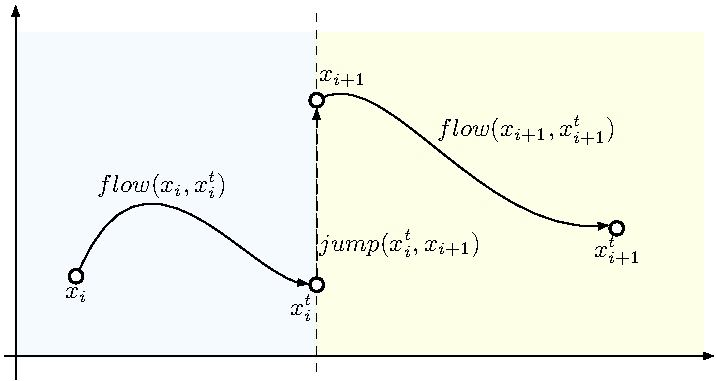
\includegraphics[width= 8cm]{deterministic.pdf}
\end{center}
\caption{}
\end{figure}

\paragraph{Systems with invariants and deterministic flows.} When the invariants are not trivial, we need to ensure that during each continuous flow, the system always stays within the invariants.
%This requires checking, for all the time points before the discrete jumps, that the invariant condition holds.
Such checking requires universal quantification over time.
%Next, we define the encoding for general hybrid systems with nontrivial invariants.
\begin{definition}[$k$-Step Reachability, Nontrivial Invariant and Deterministic Flow]
Suppose $H$ contains invariants and only deterministic flow
, and $U$ a subset of its state space represented by $\unsafe$. The $\lrf$-formula $\reach_{H,U}(k,M)$ is defined as:
\begin{eqnarray*}
& &\exists^X \vec x_{0,q_0} \exists^X\vec x_{0,q_0}^t\cdots \exists^X\vec
x_{0,q_m}\exists^X \vec x_{0,q_m}^t\cdots\exists^X \vec x_{k,q_m}\exists^X\vec x_{k,q_m}^t\exists^{[0,M]}t_0\cdots \exists^{[0,M]}t_k.\\
& &\bigvee_{q\in Q} \Big(\init_{q}(\vec x_{0,q})\wedge \flow_{q}(\vec x_{0,q}, \vec x_{0,q}^t, t_0)\wedge \forall^{[0,t_0]}t\forall^X\vec x\;(\flow_{q}(\vec x_{0,q}, \vec x, t)\rightarrow \inv_{q}(\vec x))\Big) \\
& &\wedge \bigwedge_{i=0}^{k-1}\Big( \bigvee_{q, q'\in Q} \Big(\jump_{q\rightarrow q'}(\vec
x_{i,q}^t, \vec x_{i+1,q'})\wedge \flow_{q'}(\vec x_{i+1,q'}, \vec x_{i+1,q'}^t, t_{i+1})\\
& &\hspace{6.3cm}\wedge \forall^{[0,t_{i+1}]}t\forall^X\vec x(\flow_{q'}(\vec x_{i+1,q'}, \vec x,
t)\rightarrow \inv_{q'}(\vec x)) )\Big)\Big)\\
& &\wedge\bigvee_{i=0}^k\bigvee_{q\in Q} \unsafe_q(\vec x_{k,q}^t).
\end{eqnarray*}
\end{definition}
The extra universal quantifier for each continuous flow expresses the requirement that for all the time points between the initial and ending time point ($t\in[0,t_i+1]$) in a flow, the continuous variables $\vec x$ must take values that satisfy the invariant conditions $\inv_q(\vec x)$.

\paragraph{Systems with invariants and nondeterministic flows.} In the most general case, a hybrid system can contain nondeterministic flow. When that is the case, for each time point, there is multiple possible values for the continuous variable. Yet it is not correct to universally quantify over all such possible values, because only one trajectory is needed. This problem is solved by introducing an additional level of existential quantification.
\begin{definition}[$k$-Step reachability, Nontrivial Invariant, Nondeterministic Flow]
Suppose $H$ contains invariants and nondeterministic flow, and $U$ a subset of its state space represented by $\unsafe$. The $\lrf$-formula $\reach_{H,U}(k,M)$ is defined as:
\begin{eqnarray*}
& &\exists^X \vec x_{0,q_0} \exists^X\vec x_{0,q_0}^t\cdots \exists^X\vec
x_{0,q_m}\exists^X \vec x_{0,q_m}^t\cdots\exists^X \vec x_{k,q_m}\exists^X\vec x_{k,q_m}^t\exists^{[0,M]}t_0\cdots \exists^{[0,M]}t_k.\\
& &\bigvee_{q\in Q} \Bigg(\init_{q}(\vec x_{0,q})\wedge \flow_{q}(\vec x_{0,q}, \vec x_{0,q}^t, t_0) \\
& &\hspace{1.5cm}
\wedge\forall^{[0,t_0]}t\forall^{[t,t_0]}t' \exists^X\vec x\exists^X\vec x'\\
& &\hspace{1.5cm}\Big(\inv_{q}(\vec x)\wedge \inv_{q}(\vec x')\flow_{q}(\vec x, \vec x',(t'-t))\wedge \flow_{q}(\vec x_{0, q}, \vec x, t)\wedge \flow_{q}(\vec x', \vec x^t_{0,q}, t')\Big)\Bigg) \\
& &\wedge
\bigwedge_{i=0}^{k-1}\Bigg( \bigvee_{q, q'\in Q} \Big(\jump_{q\rightarrow q'}(\vec
x_{i,q}^t, \vec x_{i+1,q'})\wedge \flow_{q'}(\vec x_{i+1,q'}, \vec x_{i+1,q'}^t, t_{i+1})\\
& &\hspace{1.5cm}
\wedge \forall^{[0,t_{i+1}]}t\forall^{[t,t_{i+1}]}t'\exists^X\vec  x\exists^X \vec  x'\\
& &\hspace{1.5cm}\Big(\inv_{q'}(\vec x)\wedge \inv_{q'}(\vec x')\wedge\flow_{q'}(\vec x, \vec x', (t'-t))\wedge \flow_{q'}(\vec x_{i+1, q'}, \vec x, t)\wedge \flow_{q'}(\vec x', \vec x^t_{i+1,q'}, t')\Big)\Bigg)\\
& &\wedge\ \bigvee_{i=0}^k\bigvee_{q\in Q} \unsafe_q(\vec x_{k,q}^t).
\end{eqnarray*}
\end{definition}


\begin{figure}[h!]
\begin{center}
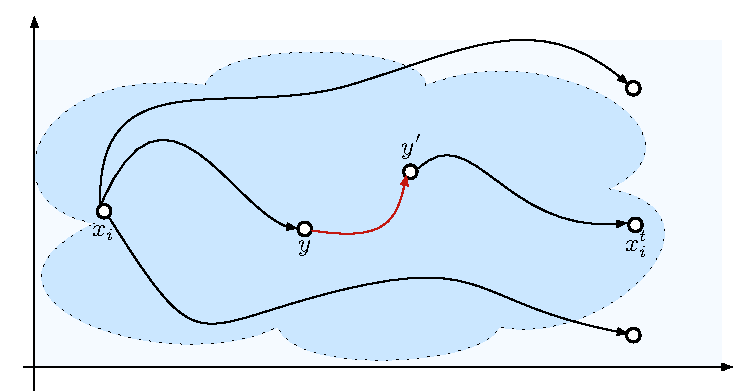
\includegraphics[width= 8cm]{nondet.pdf}
\end{center}
\caption{}
\end{figure}



Intuitively, at each time point, the innermost existential quantifier asks for an assignment to the continuous variables $\vec x$ such that: first, there is a flow from the initial state in this step to the current assignment, as encoded by $\flow_{q'}(\vec x_{i+1,q'}, \vec x,t)$; second, from the current assignment there is a flow to $\vec x^t_{i+1,q'}$, the value that the continuous variables are supposed to take after the rest of the flow.

In the next section we will use these encodings to connect between $\delta$-reachability and $\delta$-decision problems of the corresponding $\lrf$-formulas. 

\subsection{$\delta$-Complete Bounded Reachability Analysis}

\begin{lemma}\label{equiv-delta}
Let $\delta\in\mathbb{Q}^+\cup \{0\}$ be arbitrary. Suppose $H$ is a hybrid system, $U$ a subset of its state space represented by $\unsafe$, and $\reach_{H,U}(k,M)$ encodes $(k,M)$-bounded reachability. Let $H$, $U$, $k$, $M$ all be arbitrary. 

We always have $\mathbb{R}\models(\reach_{H,U}(k,M))^{\delta}$, iff, there exists a trajectory $\xi\in\llbracket H^{\delta}\rrbracket$ such that for some $(k,t)\in T^{M}(\xi)$, $(\xi(k, t), \sigma_{\xi}(k))\in \llbracket \unsafe^{\delta}\rrbracket$.
\end{lemma}

\begin{proof}
We prove by induction on $k$, for the most general case of systems with nontrivial invariants and nondeterministic flows. The simpler cases then automatically hold.

(i) Case $k=0$. Suppose $\reach^{\delta}_{H,U}(0,M)$ is true. Then there exists $q\in Q$, $\vec a_0, \vec a_0^t\in \mathbb{R}^n\cap X$ and $t_0\in\mathbb{R}^+\cap[0, M]$ such that for all $t\in [0,t_0]$, there exists $\vec a(t)\in X$ satisfying:
\begin{multline*}
\init_{q}^{\delta}(\vec a_0)\wedge\flow_{q}^{\delta}(\vec a_0, \vec a_0^t, t_0)
\wedge \flow_q^{\delta}(\vec a_0, \vec a(t), t) \wedge \flow^{\delta}_q(\vec a(t), \vec a_t, t_0-t)\wedge \inv_q(\vec a(t)) \wedge \unsafe^{\delta}_q(\vec a_t).
\end{multline*}
Note that there is no discrete jump. Accordingly, set a trajectory $\xi$ to be: 
$$\xi(0,0) = \vec a_0, \xi(0,t_0) = \vec a_0^t,$$
and for all time point $t\in [0,t_0]$, $\xi(0,t)\in \vec a(t)$. Following Definition~\ref{trajec} and Definition~\ref{lrf-definition}, $\xi\in\llbracket H^{\delta}\rrbracket$, and $\xi(0, \vec a_0^t)\in\llbracket \unsafe^{\delta}\rrbracket$.

On the other hand, suppose there is a $\xi\in \llbracket H^{\delta}\rrbracket$ such that $\xi(0,t_0)$ is in $\llbracket\unsafe_q\rrbracket$ for some $t_0\in[0,M]$. We set $\vec a_0 = \xi(0,0)$, $\vec a_0^t = \xi(0,t_0)$. Then following the conditions that $\xi$ satisfies in Definition~\ref{trajec}, for every $t\in [0,t_0]$, there is $\vec a(t)$ such that $\flow^{\delta}_q(\vec a_0,\vec a(t),t)$ and $\flow^{\delta}_q (\vec a(t), \vec a_t, t)$. Consequently, $\reach_{H,U}^{\delta}(0,M)$ is true, witnessed by these assignments.

(ii) Case $k \geq 1$. Suppose $\reach^{\delta}_{H,U}(k,M)$ is true. Then there exists 
$$q_0, ... ,q_{k}\in Q, \vec a_{0}, \vec a_{0}^t, ... ,\vec a_{k}, \vec a_{k}^t \in X,\mbox{ and } t_0,...,t_k\in[0, M]$$ such that for all $t_{q_0}\in [0,t_0],...,t_{q_k}\in [0,t_k]$ there exists $\vec a(t_{q_0}),...,\vec a(t_{q_k})\in X$ satisfying:
\begin{eqnarray*}\label{kstep}
& &\init_{q}^{\delta}(\vec a_0)\wedge\flow_{q}^{\delta}(\vec a_{0}, \vec a_0^t, t_0) \wedge \flow_q^{\delta}(\vec a_0, \vec a(t), t)\wedge \flow^{\delta}_{q_0}(\vec a(t), \vec a_0^t, t_0-t)\wedge \inv^{\delta}_{q_0}(\vec a(t))\\
& & \wedge \jump^{\delta}_{q_0\rightarrow q_1}(\vec a_0^t, \vec a_1)\wedge\cdots\wedge \flow_{q_{k-1}}^{\delta}(\vec a_{k-1}, \vec a_{k-1}^t, t_0)
\wedge\flow_{q_{k-1}}^{\delta}(\vec a_{k-1}, \vec a(t_{q_{k-1}}), t)\\
& &\wedge \flow^{\delta}_{q_{k-1}}(\vec a(t_{q_{k-1}}), \vec a_k^t, (t_{k-1}-t))\wedge \inv^{\delta}_{q_{k-1}}(\vec a(t_{q_{k-1}}))\\
& &\wedge \jump^{\delta}_{q_{k-1}\rightarrow q_k}(\vec a_{k-1}^t, \vec a_k)\wedge \flow_{q_{k}}^{\delta}(\vec a_{k}, \vec a_{k}^t, t_k)
\wedge\flow_{q_{k}}^{\delta}(\vec a_{k}, \vec a(t_{q_{k}}), t_k)\\
& &\wedge \flow^{\delta}_{q_{k}}(\vec a(t_{q_{k-1}}), \vec a_k^t, (t_{q_{k-1}}-t))\wedge \inv^{\delta}_{q_{k-1}}(\vec a(t_{q_{k}}))\wedge \unsafe^{\delta}_{q_k}(\vec a_k^t).
\end{eqnarray*}
Now, to perform induction, we truncate the last step in the formula and define a new region $U'$ represented by:
\begin{eqnarray*}
\unsafe^{\mathrm{tail}}_{q_{k-1}}(\vec x) &=& \jump_{q_{k-1}\rightarrow q_k}(\vec x, \vec a_k)\wedge \flow_{q_{k}}(\vec a_{k}, \vec a_{k}^t, t_k)\wedge\flow_{q_{k}}(\vec a_{k}, \vec a(t_{q_{k}}), t_k)\\
& &\wedge \flow_{q_{k}}(\vec a(t_{q_{k-1}}), \vec a_k^t, (t_{q_{k-1}}-t))\wedge \inv_{q_{k-1}}(\vec a(t_{q_{k}}))\wedge \unsafe_{q_k}(\vec a_k^t).
\end{eqnarray*}
%$U' = q_{k-1}, \llbracket \unsafe^{\mathrm{tail}}_{q_{k-1}}(\vec x)\rrbracket$.
We then see that the formula
$\reach_{H, U'}^{\delta}(k-1, M)$
is true, as simply witnessed by the trace above, using the new formula $\unsafe^{\mathrm{tail}}_{q_{k-1}}$ to represent the last transition:
\begin{eqnarray*}\label{kstep}
& &\init_{q}^{\delta}(\vec a_0)\wedge\flow_{q}^{\delta}(\vec a_{0}, \vec a_0^t, t_0) \wedge \flow_q^{\delta}(\vec a_0, \vec a(t), t)
\wedge \flow^{\delta}_{q_0}(\vec a(t), \vec a_0^t, t_0-t)\wedge \inv^{\delta}_{q_0}(\vec a(t))\\
& & \wedge \jump^{\delta}_{q_0\rightarrow q_1}(\vec a_0^t, \vec a_1)\wedge\cdots\wedge \flow_{q_{k-1}}^{\delta}(\vec a_{k-1}, \vec a_{k-1}^t, t_0)
\wedge\flow_{q_{k-1}}^{\delta}(\vec a_{k-1}, \vec a(t_{q_{k-1}}), t)\\
& &\wedge \flow^{\delta}_{q_{k-1}}(\vec a(t_{q_{k-1}}), \vec a_k^t, (t_{k-1}-t))\wedge \inv^{\delta}_{q_{k-1}}(\vec a(t_{q_{k-1}}))\wedge(\unsafe_{q_{k-1}}^{\mathrm{tail}}(\vec a_{k-1}^t))^{\delta}.
\end{eqnarray*}
Consequently, by inductive hypothesis, there exists a trajectory $\xi_{k-1}\in\llbracket H^{\delta}\rrbracket$ that reaches the region $U'$. Now, we extend $\xi_{k-1}$ with the assignments in the $k$-the step, i.e.:
$$\xi = \xi_{k-1}\cup\{(k,\vec a(t_{q_k})): t\in [0,t_k]\}$$
where $\vec a(0) = \vec a_k, \vec a(t_k)=\vec a_k^t$. We now obtain $\xi\in \llbracket H^{\delta}\rrbracket$ such that $\xi$ reaches the region represented by $\unsafe^{\delta}$.

On the other hand, suppose there is a trajectory $\xi\in\llbracket H^{\delta}\rrbracket$ such that $\xi$ reaches the region represented by $\unsafe^{\delta}$. Again, following an argument similar to the above, and Definition~\ref{trajec} we can find the sequence of assignments that witnesses the formula $\reach^{\delta}_{H,U}(k,M)$ to be true.
\end{proof}
Now we can easily show that the bounded $\delta$-reachability problems is decidable for any $\lrf$-representable hybrid system.
\begin{theorem}[Decidability]
Let $\delta\in \mathbb{Q}^+$ be arbitrary. There exists an algorithm such that, for any hybrid system $\lrf$-represented by $H$ and an unsafe region $U$ $\lrf$-represented by $\unsafe$, solves the $(k,M)$-bounded $\delta$-reachability problem for $H$ for any given bounds $k\in \mathbb{N}, M\in \mathbb{R}^+$.
\end{theorem}
\begin{proof}
We need to show that there is an algorithm that correctly returns one of the following answers:
\begin{itemize}
\item {\sf safe:} $H$ does not reach the region represented by $\unsafe$ within the $(k,M)$-bound;
\item {\sf $\delta$-unsafe:} $H^{\delta}$ reaches the region represented by $\unsafe^{\delta}$ within the $(k,M)$-bound.
\end{itemize}
For this, we only need to solve the $\delta$-decision problem for the formula $\reach^k_{H,U}(i,M)$, from which we obtain an answer of either $\varphi$ is false, or $\varphi$ is $\delta$-true (Theorem~\ref{delta-decide}).

$\bullet$ Suppose $\varphi$ is false. Then we know that for any $i\leq k$, $\reach_{H,U}(i,M)$ is false. Using Lemma~\ref{equiv-delta} for the special case $\delta=0$, we know that there does not exist a trajectory $\xi\in\llbracket H\rrbracket$ that can reach $U$ within $i$ steps, and consequently the system is safe within the $(k,M)$-bound.

$\bullet$ Suppose $\varphi$ is $\delta$-true, we know that there exists $i\leq k$ such that $\reach^{\delta}_{H,U}(i,M)$ is true. Using Lemma~\ref{equiv-delta} for $\delta\in\mathbb{Q}^+$, we know that there exists a trajectory $\xi\in\llbracket H^{\delta}\rrbracket$ that can reach the region represented by $\unsafe^{\delta}$ in $i$-steps, i.e., within the $(k,M)$-bound.
\end{proof}

From the structures of the $\lrf$-formulas encoding $\delta$-reachability, we can obtain the following complexity results of the reachability problems.
\begin{theorem}[Complexity]
Suppose all the functions in the description of $H$ is in complexity class $\mathsf{C}$. Then deciding the $(k,M)$-bounded $\delta$-reachability problem is in
\begin{itemize}
\item $\np^{\mathsf{C}}$ for an invariant-free $H$;
\item $(\Sigma_2^P)^{\mathsf{C}}$ for $H$ with nontrivial invariants and deterministic flows;
\item $(\Sigma_3^P)^{\mathsf{C}}$ for $H$ with nontrivial invariants and nondeterministic flows.
\end{itemize}
\end{theorem}
\begin{proof}
It is clear that the logic structures of the $\reach_{H,U}(k,M)$ formulas in the three cases are $\Sigma_1$, $\Sigma_2$, and $\Sigma_3$ respectively. Consequently, using complexity results for Theorem~\ref{compmain}, the complexity of the $\delta$-decision problems resides in $\np^{\mathsf{C}}$, $(\Sigma_2^P)^{\mathsf{C}}$, and $(\Sigma_3^P)^{\mathsf{C}}$ respectively.

The missing step here is that the $\reach_{H,U}(k,M)$ formulas are of exponential length, because of the enumeration of all possible paths through the discrete modes requires an exponential number ($m^{k+1}$, where $m$ is the number of discrete modes in $H$) of copies of the continuous variables. Thus the $\reach_{H,U}(k,M)$ encodings do not provide a polynomial-reduction to the $\delta$-decision problems.

Observe that, however, we can nondeterministically select single paths through the modes. This is just what we did in the proof of Lemma~\ref{equiv-delta}. Here we show how to do this for the $\Sigma_3$ case of nontrivial invariants and nondeterministic flows and the other cases are subsumed. Nondeterministically, we can choose a sequence of modes $q_0,...,q_k\in Q$ and solve the $\delta$-decision problem for the formula:
\begin{eqnarray*}
& &\exists^X \vec x_0 \exists^X \vec x_0^t\cdots \exists^X \vec x_q \exists^X \vec x_q^t
\exists^{[0,M]} t_0\cdots \exists^{[0,M]} t_k\forall^{[0,t_0]}t_{q_0} \cdots \forall^{[0,M]} t_{q_k}\exists^X
x_{q_0}\cdots\exists\vec x_{q_{k}}\\
& & \Big(\init(\vec x_0)\wedge \flow_{q_0}(\vec x_0, \vec x_0^t, t_0)\wedge \flow_{q_0}(\vec x_0, \vec x_{q_0}, t_{q_0})\wedge \flow_{q_0}(\vec x_{q_0}, \vec x_0^t, (t_0-t_{q_0}))\\
& &\wedge\inv_{q_0}(\vec x_{q_0})\wedge \jump_{q_0\rightarrow q_1}(\vec x_0', \vec x_1)\wedge \cdots\wedge \flow_{q_k}(\vec x_k, \vec x_{q_k}, t_{q_k})\wedge \flow_{q_k}(\vec x_{q_k}, \vec x_k^t, (t_k-t_{q_k}))\\
& &\wedge\inv_{q_k}(\vec x_{q_k})\wedge\unsafe_{q_k}(\vec x_k^t)\Big)
\end{eqnarray*}
Now, this formula is polynomial in $H$, $\unsafe$, $k$, $M$. Thus, we can use the
nondeterministic machine to randomly first select such a formula in polynomial
time, and $\delta$-decide its truth value, which is in $\mathsf{(\Sigma_3^P)^C}$. Thus, the complexity of the $\delta$-reachability problem is still in $\mathsf{(\Sigma_3^P)^C}$ for this case.
\end{proof}

\begin{corollary}
For linear and polynomial hybrid automata, the bounded $\delta$-reachability problem ranges from being $\mathsf{NP}$-complete to $\mathsf{\Sigma_3^P}$-complete for the three cases. For hybrid automata that can be $\lrf$-represented with whose $\mathcal{F}$ contains the set of ODEs defined $\mathsf{P}$-computable right-hand side functions, the problem is $\mathsf{PSPACE}$-complete.
\end{corollary}
\begin{proof}
The results come from the fact that the complexity of polynomials is in $\mathsf{P}$, and the set of ODEs in questions are $\mathsf{PSPACE}$-complete.
\end{proof}
\bibliographystyle{abbrv}
\bibliography{tau}
\newpage

\end{document}

